\section{Method of Regularized Stokeslets}

\begin{equation}
\label{eq:blobfunc}
    \phi_\epsilon(\mathbf{x})= \frac{15 \epsilon^4}{8\pi\left( |\mathbf{x}|^2 +\epsilon^2 \right)^{7/2}}
\end{equation}

\begin{figure}[h]
    \centering
    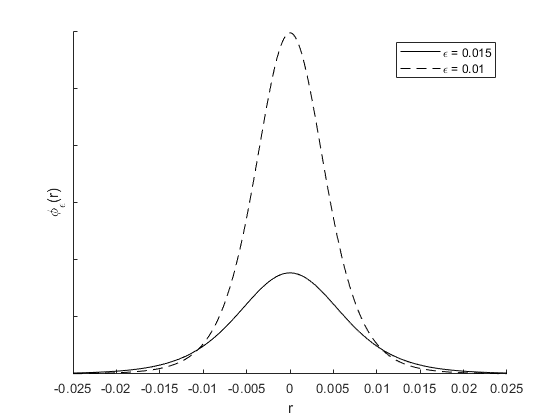
\includegraphics[scale=0.65]{Images/BlobFunction.png}
    \caption{Blob function in equation Eq.\eqref{eq:blobfunc} for several values of epsilon}
    \label{fig:blobfunc}
\end{figure}

\begin{subequations}
\label{eq:RegStokesFlow}
\begin{align}
    \mu\Delta\boldsymbol{u} &= \nabla p - \phi_{\varepsilon}(\mathbf{x})\mathbf{f_0} \label{eq:RegStokesFlow1} \\ 
    \nabla \cdot \boldsymbol{u} &= 0 \label{eq:RegStokesFlow2}
\end{align}
\end{subequations}

\begin{subequations}
\label{eq:intermediate}
\begin{align}
    \Delta G_\varepsilon  &= \phi_\varepsilon(\mathbf{x}) \label{eq:inter1} \\
    \Delta B_\varepsilon  &= G_\varepsilon \label{eq:inter2}
\end{align}
\end{subequations}

\begin{equation}
    \mu \mathbf{u} = (\mathbf{f_0}\cdot\nabla)\nabla\mathbf{B_\varepsilon}(\mathbf{x}-\mathbf{x_0})-\mathbf{f_0}\mathbf{G_\varepsilon}(\mathbf{x}-\mathbf{x_0})
\end{equation}

\begin{equation}
\label{eq:regstokeslet1}
    s_{ij}^\varepsilon(\mathbf{x}, \mathbf{x_0}) = 8\pi\left[ \frac{\partial^2 B(\mathbf{x} -\mathbf{x_0})}{\partial x_i \partial x_j} - \delta_{ij}  G(\mathbf{x} -\mathbf{x_0})\right]
\end{equation}

\begin{equation}
\label{eq:regstokeslet2}
    s_{ij}^\varepsilon(\mathbf{x}, \mathbf{x_0})   = \delta_{ij} \frac{r^2+2\varepsilon^2}{\left( r^2 + \varepsilon^2 \right)^{3/2}} + \frac{(x_i-x_{0i})(x_j-x_{0j})}{\left( r^2 + \varepsilon^2 \right)^{3/2}}
\end{equation}
where $r=|\mathbf{x}-\mathbf{x_0}|$. 

\begin{equation}
    \int_{\mathbb{R}^{3}} u_{j}(\mathbf{x}) \phi_{\epsilon}\left(\mathbf{x}-\mathbf{x}_{0}\right) d V(\mathbf{x})=-\frac{1}{8 \pi \mu} \int_{\partial D} S_{i j}^{\epsilon}\left(\mathbf{x}, \mathbf{x}_{0}\right) f_{i} d s(\mathbf{x})
\end{equation}


\begin{equation}
\label{eq:Stokesletsum}
    u_{j}\left(\mathbf{x}_{0}\right)=\frac{1}{8 \pi \mu} \sum_{n=1}^{N} \sum_{i=1}^{3} S_{i j}^{\epsilon}\left(\mathbf{x}_{n}, \mathbf{x}_{0}\right) f_{n, i} A_{n}
\end{equation}